%!TEX root = ../march2025poster.tex

\begin{block}{Results so far (cont.)}
\begin{center}
	\begin{figure}
		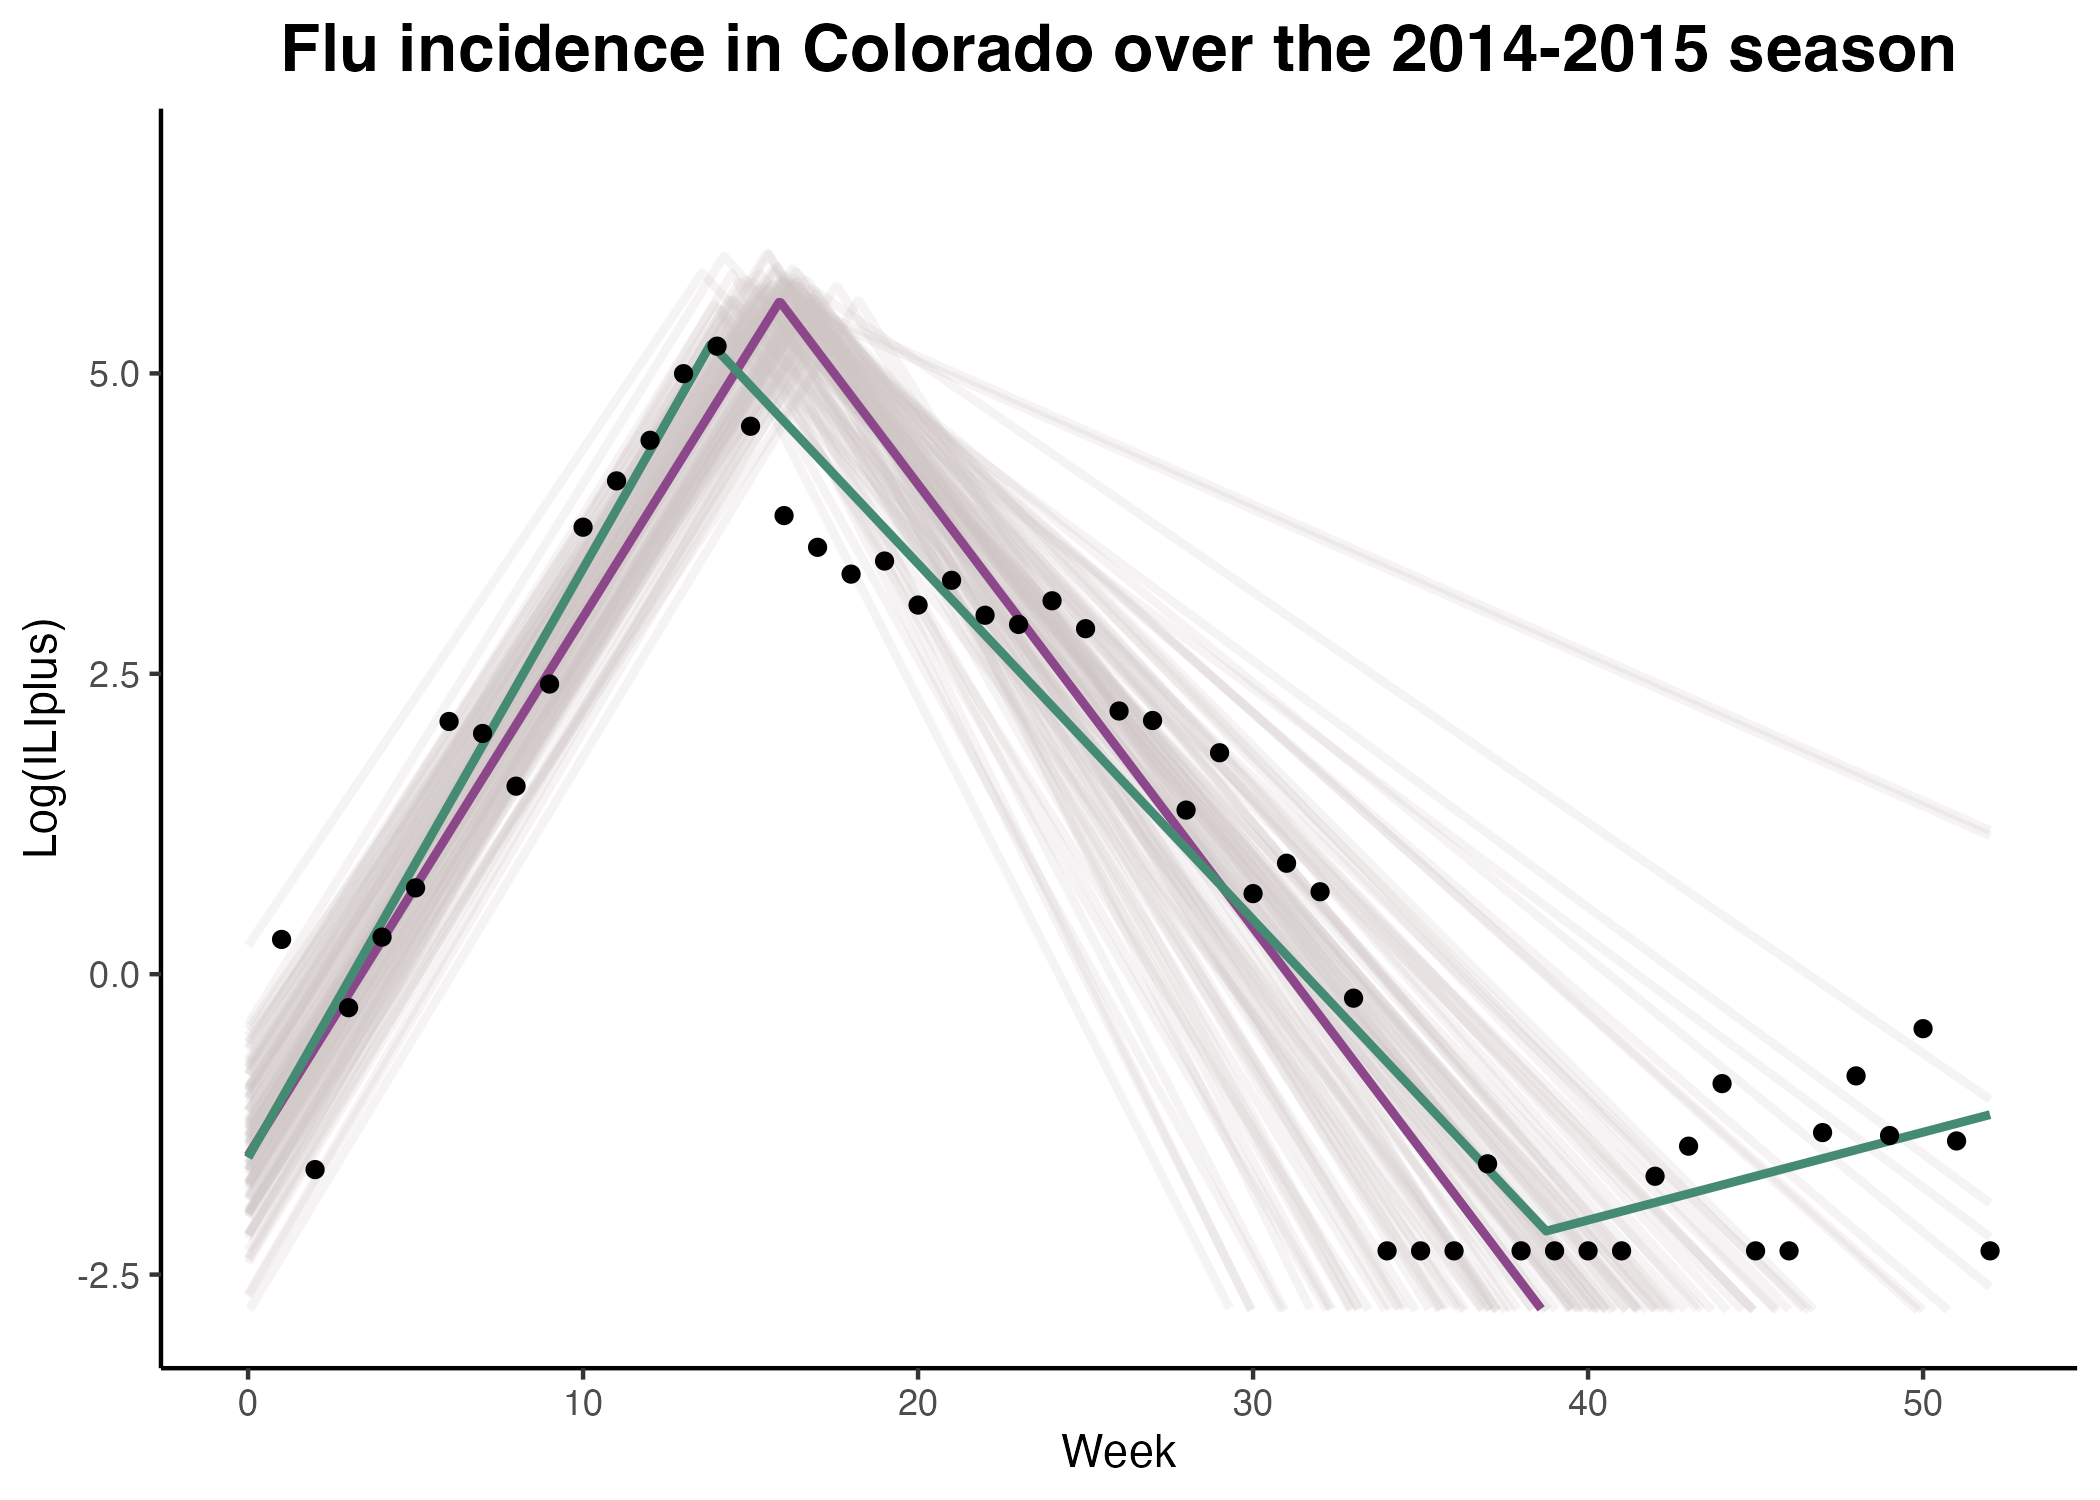
\includegraphics[width = 0.48\columnwidth]{sections/images/Colorado2014.png}
		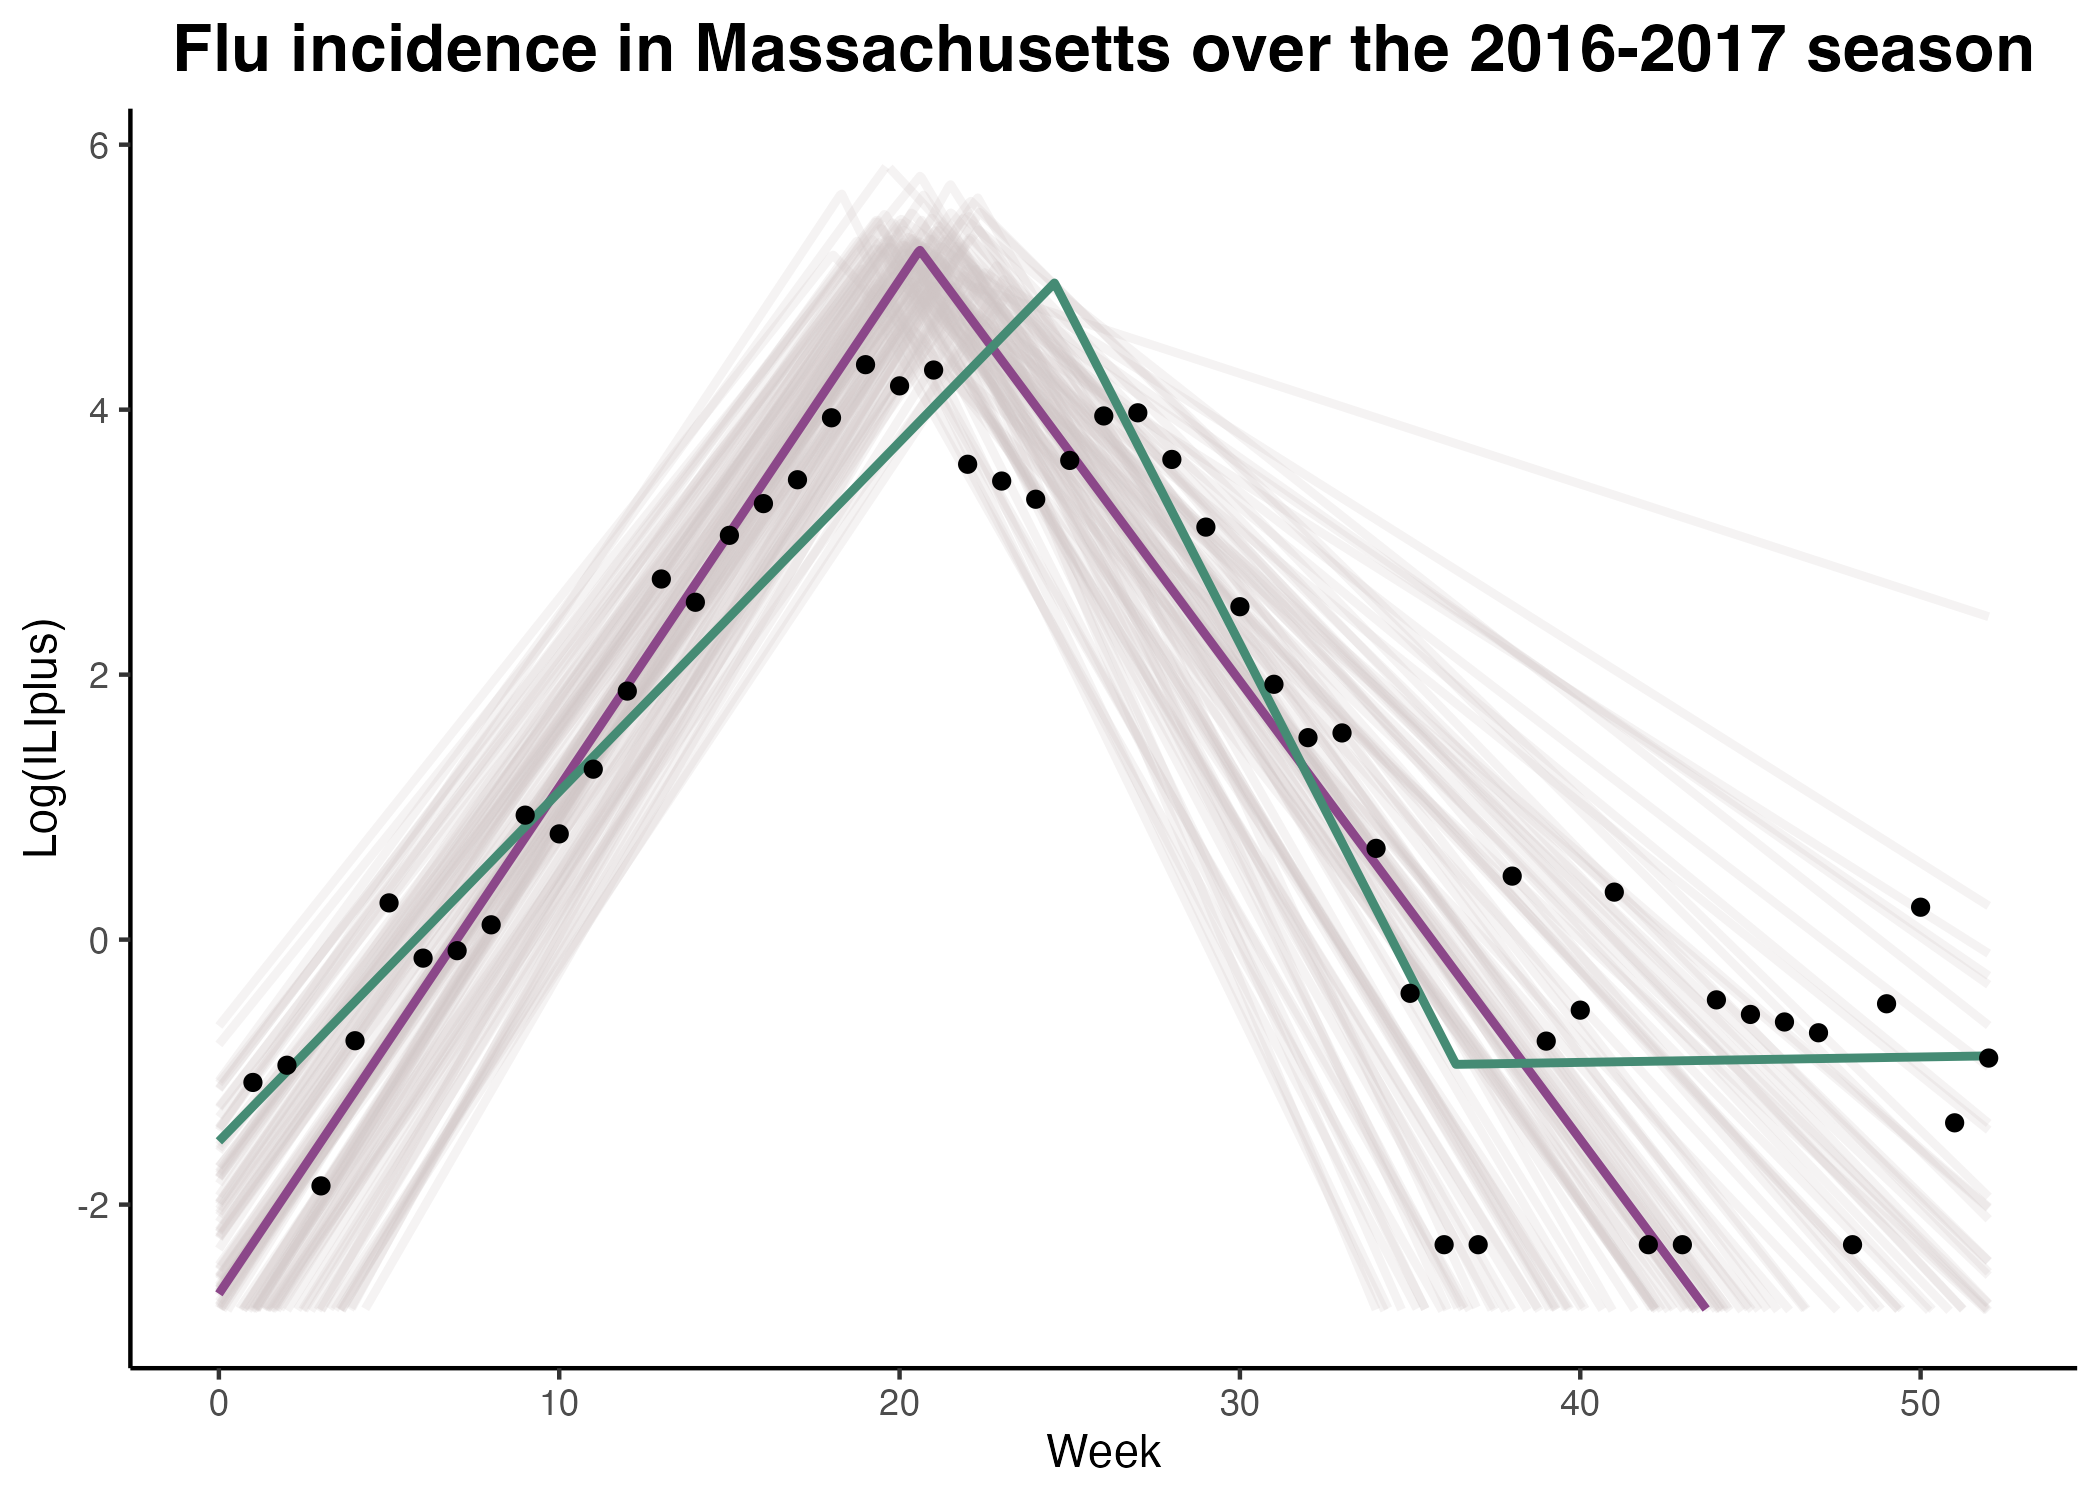
\includegraphics[width = 0.48\columnwidth]{sections/images/Massachusetts2016.png}
		\\
		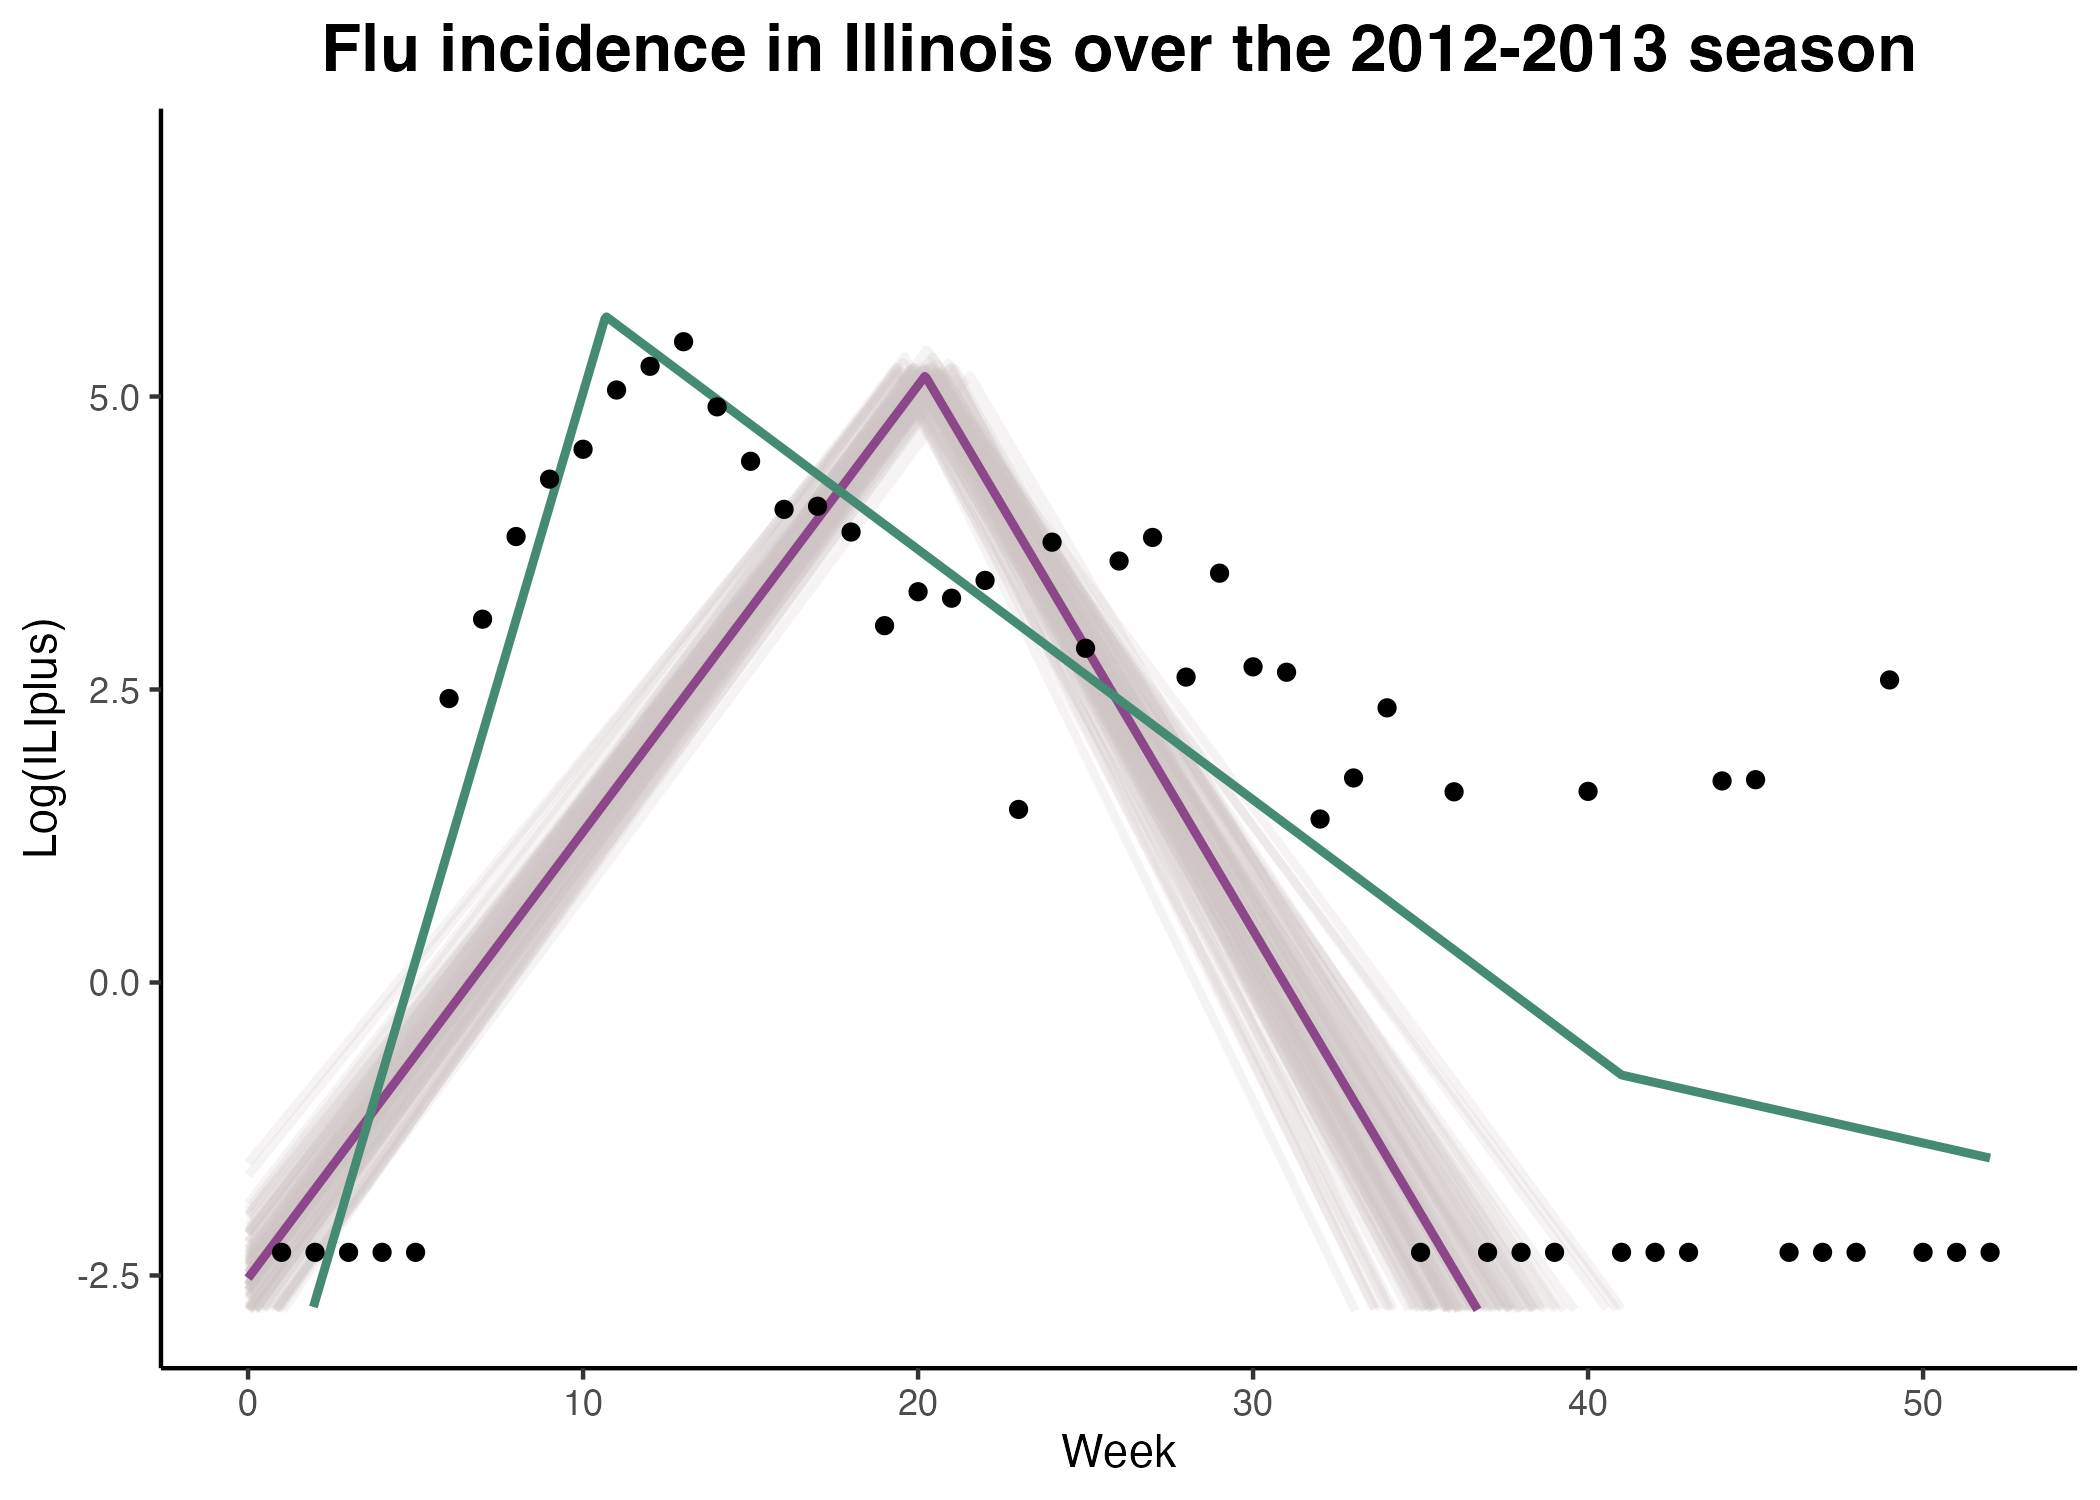
\includegraphics[width = 0.48\columnwidth]{sections/images/Illinois2012.png}
		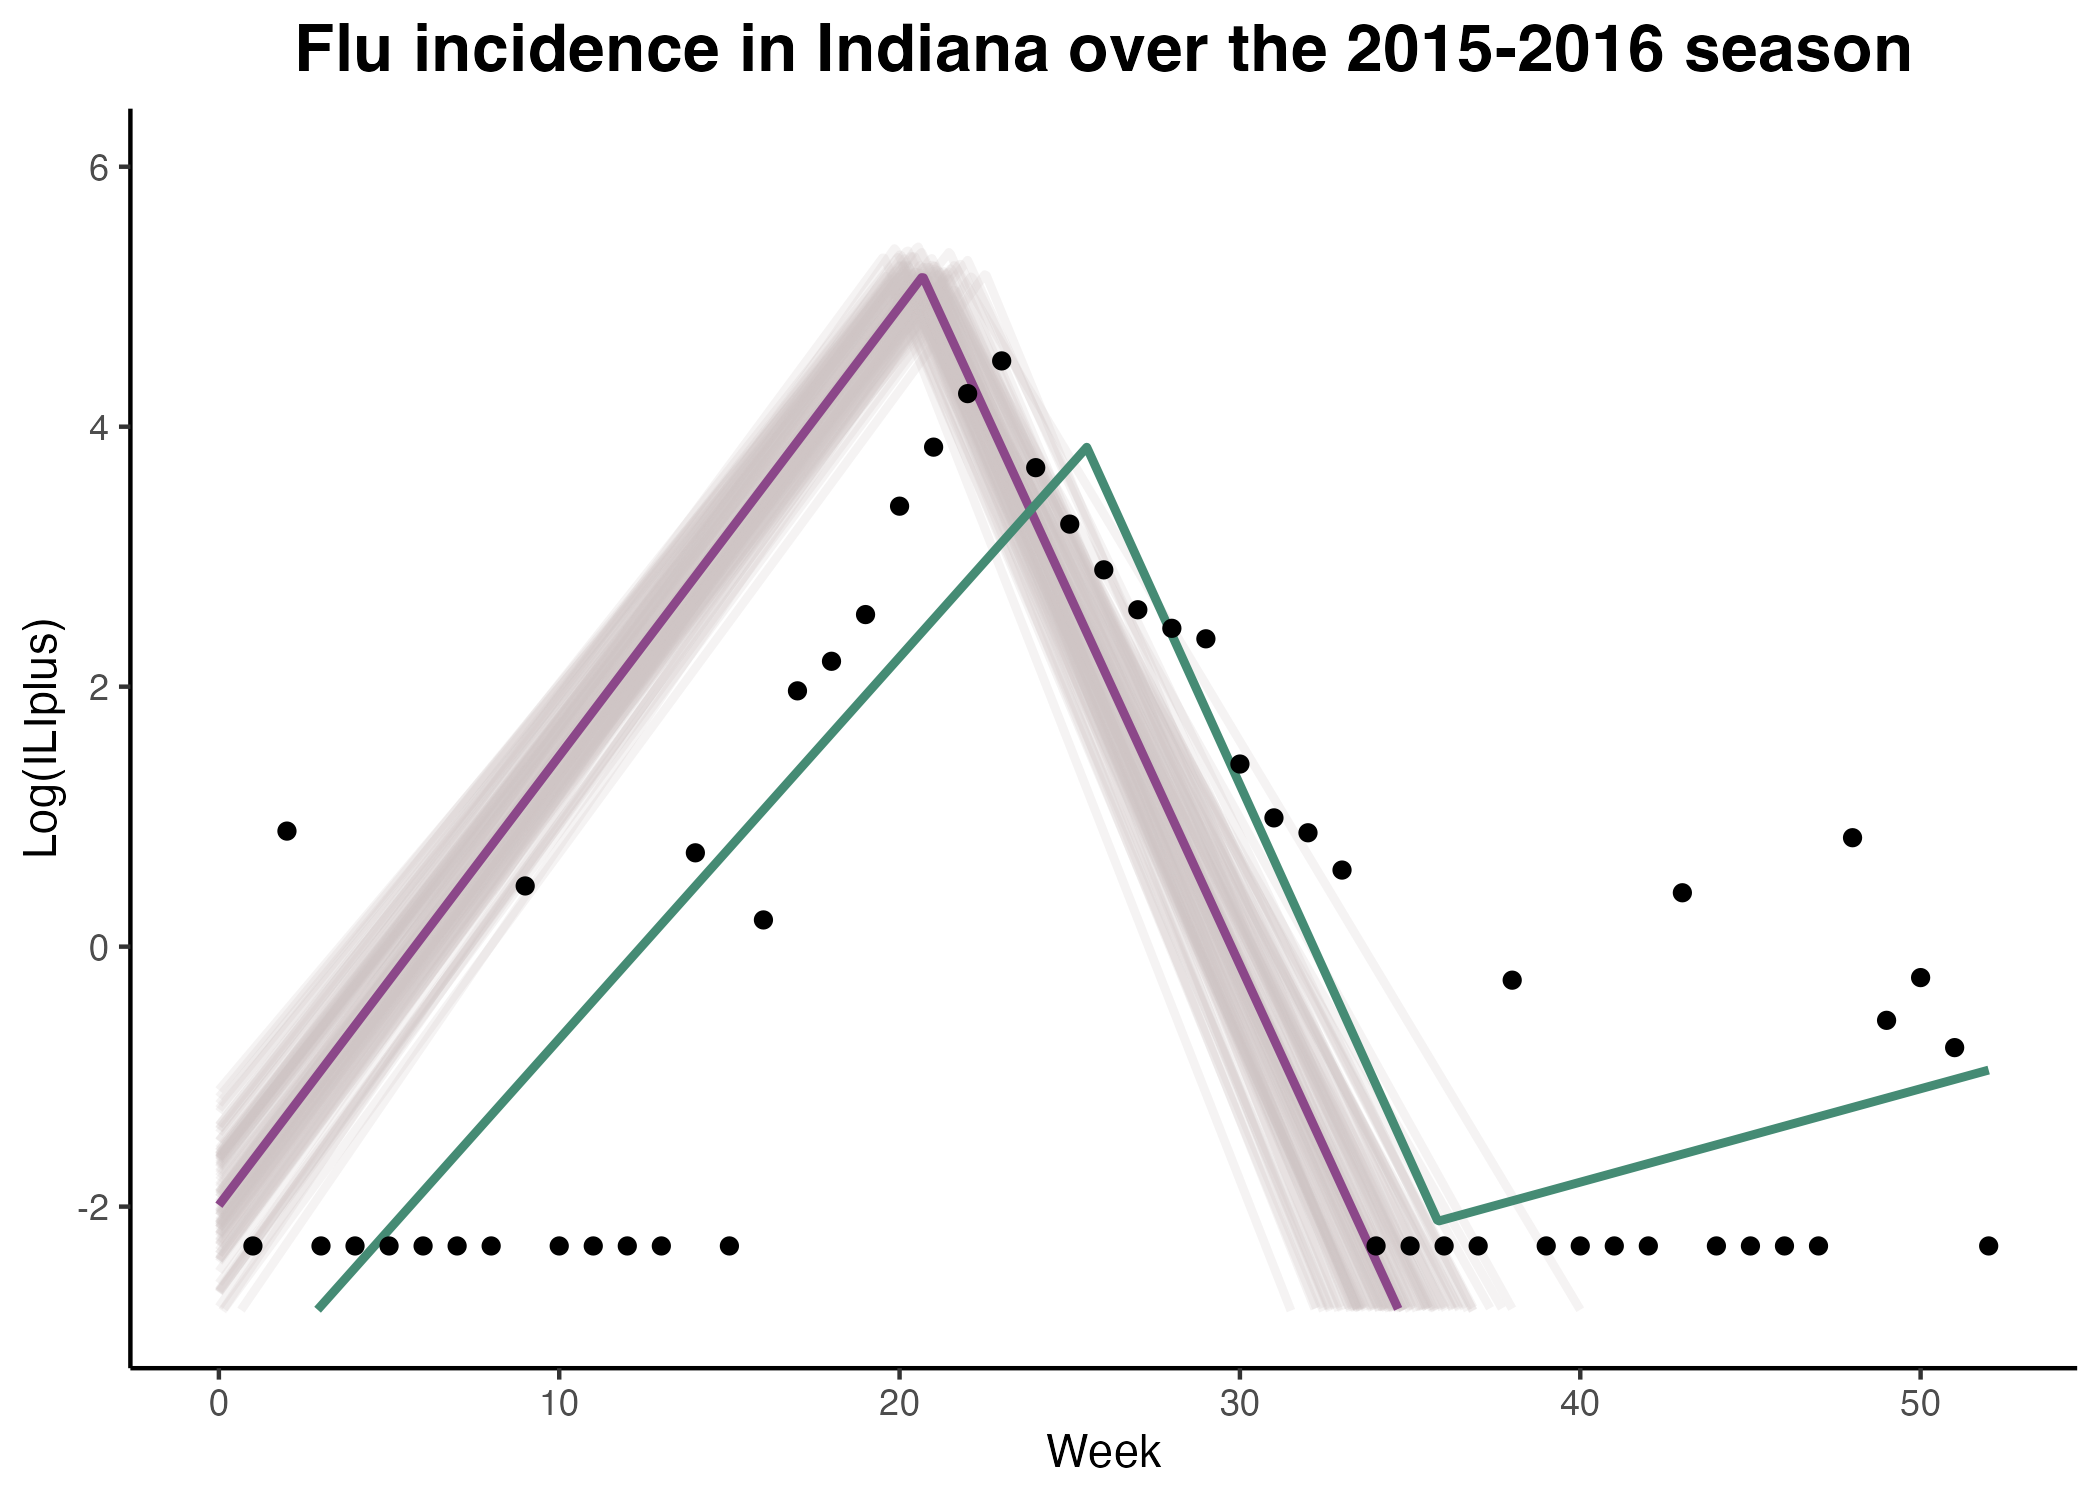
\includegraphics[width = 0.48\columnwidth]{sections/images/Indiana2015.png}\\
		\caption{Flu incidence in four different states and years along with the piecewise linear fit (green line) and the piecewise linear fits predicted by that state/year's climate and population data (mean of posterior distribution - purple line, 100 draws from posterior distribution - light purple lines).}
	\end{figure}
\end{center}
\begin{itemize}
	\item Some predicted fits are quite good! 
	\item Others are not as good
	\item In general, the Bayesian model parameter predictions have less variance than the true parameters (up slope, down slope, etc.)
\end{itemize}
\end{block}
\vspace{\colthreesep}

\begin{block}{Future Work}
	\begin{itemize}
		\item Consider other climate variables (e.g. minimum temperature) and timing of climate variables (i.e. we'd expect the temperature, humidity, etc. earlier in the season to have a greater impact)
		\item Model evaluation and comparison 
		\item Implement Bayesian *hierarchical* modeling
		\item Actually create forecasts using an ARIMA (autoregressive integrated moving average) model 
	\end{itemize}
\end{block}

\vspace{\colthreesep}

\begin{block}{References}
	\leftskip 01in
	\parindent -01in
	[1] Bracher, Johannes. "On the multibin logarithmic score used in the FluSight competitions."\textit{ Proceedings of the National Academy of Sciences} 116.42 (2019): 20809-20810. \\
	\vspace{.75ex}
	[2] du Prel, Jean-Baptist, et al. "Are meteorological parameters associated with acute respiratory tract infections?." \textit{Clinical infectious diseases} 49.6 (2009): 861-868. \\
	\vspace{.75ex}
	[3] Frongillo, Rafael M. \textit{Eliciting private information from selfish agents}. University of California, Berkeley, 2013. \\
	\vspace{.75ex}
	[4] Goldstein, Edward, et al. "Predicting the epidemic sizes of influenza A/H1N1, A/H3N2, and B: a statistical method." \textit{PLoS medicine} 8.7 (2011): e1001051. 

\end{block}

